\chapter{Исследовательская часть}

В данном разделе представлено сравнение времени агрегации данных в OLAP Cube при разном количестве результатов, показанных на Олимпийских играх.

\section{Постановка эксперимента}

Время обработки замерялось при помощи библиотеки time. Время замерялось на протяжении 100 запусков и брался средний показатель.

\subsection{Цель эксперимента}

Целью эксперимента является сравнение времени, требуемого для агригации полученных данных.

\subsection{Результат эксперимента}

В таблице \ref{tbl:experiment} представлены результаты поставленного эксперимента.

\begin{table}[H]
	\centering
	\caption{Результаты сравнения времени, необходимого для агрегации данных Олимпиад}
	\label{tbl:experiment}
	\resizebox{\textwidth}{!}{%
		\begin{tabular}{|l|l|l|}
			\hline
			\textbf{\begin{tabular}[c]{@{}c@{}}Количество \\ результатов\end{tabular}} & \textbf{Количество cрезов (slice) по осям} & \textbf{Время , мс} \\ \hline
			100 & 0 & 1490 \\ \hline
			100 & 1 & 989 \\ \hline
			100 & 2 & 300 \\ \hline
			500 & 0 & 1561 \\ \hline
			500 & 1 & 1000 \\ \hline
			500 & 2 & 490 \\ \hline
			1500 & 0 & 1763 \\ \hline
			1500 & 1 & 1100 \\ \hline
			1500 & 2 & 621 \\ \hline
			3000 & 0 & 2167 \\ \hline
			3000 & 1 & 1700 \\ \hline
			3000 & 2 & 1121 \\ \hline
			3000 & 3 & 1000 \\ \hline
			5000 & 0 & 2727 \\ \hline
			5000 & 1 & 1500 \\ \hline
			5000 & 2 & 1100 \\ \hline
			5000 & 3 & 570 \\ \hline
			10000 & 0 & 3476 \\ \hline
			10000 & 1 & 2056 \\ \hline
			10000 & 2 & 1302 \\ \hline
			10000 & 3 & 811 \\ \hline
		\end{tabular}%
	}
\end{table}

На рисункt \ref{ing:graph} представлены графики зависимости времени агрегации от количества результатов, показанных на Олимпийских играх.

\newpage
\begin{figure}[!h]
	\center{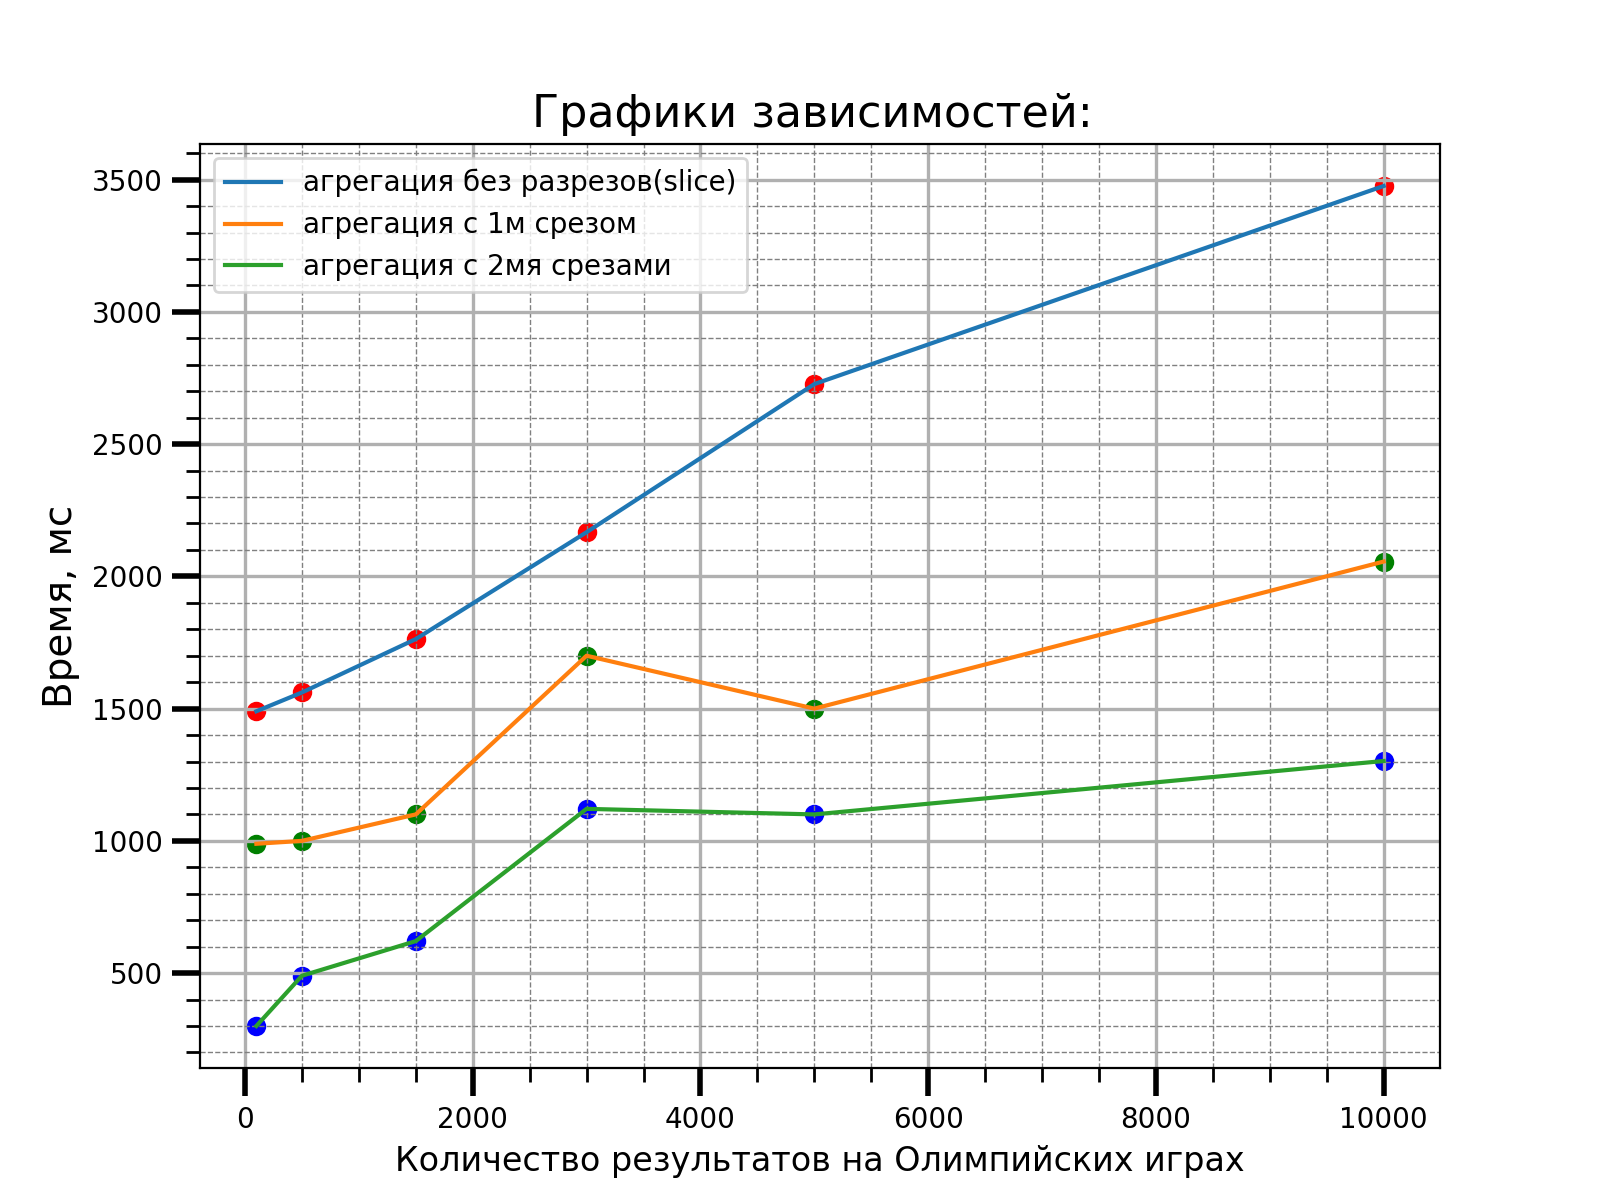
\includegraphics[scale=0.8]{img/graph.png}}
	\caption{Зависимость времени агригации данных от количества результатов, при отсутствии, одном и двух срезах.}
	\label{ing:graph}
\end{figure}

\section*{Вывод}

В результате сравнения времени, необходимого для агрегации данных об результатах Олимпиад, были получены следующие результаты:

\begin{itemize}
	
	\item  С увелечением количества результатов Олимпиады увеличивается время агрегации;
	
	\item  С увелечением количества срезов время агрегации уменьшается;
	
	\item   С увелечением количества срезов скорость роста времени агрегации уменьшается при увелечении количества данных;
	
\end{itemize}

Выяснено, что эффективность агрегации с ростом объёма данных уменьшается при отсутствии операций среза. В тоже время при увелечении количества срезов время агрегации на тех же объёмах данных значительно сокращается и замедляет свой рост. 

Можно сделать вывод, что способ анализа и агригирования данных с помощью OLAP куба показывает максимальную эффективность при введении некоторого числа срезов. Возможно, другие OLAP модели или  иные технологии анализа могут дать лучшие результаты и без введения срезов.




